\section{Simulation and Data Sample}

The method by which all of the measurements presented in this thesis are performed is that of \emph{Monte-Carlo (MC) forward folding}. In a nutshell, this method involves producing a large set of simulated signal and background events that are then re-weighted in such a way that their distribution matches that of the observed data events as closely as possible. To give reliable results, an accurate simulation of all particle interactions described in Section~\ref{sec:particle-interactions} as well as the detector electronics described in section~\ref{sec:dom-daq} is required. The simulated and observed events are then passed through the same data processing chain described in section~\ref{sec:data-processing}. The resulting MC simulated dataset and the observed dataset are then histogrammed in the same binning, and the weights of the MC events are adjusted to give the best match between the histograms according to a loss function as defined in section~\ref{sec:test-statistic}.

The simulation chain for neutrinos and atmospheric muons can generally be divided into three steps that are described in this chapter:
\begin{enumerate}
    \item Simulation of particle interactions
    \item Photon propagation in ice
    \item Response of detector DAQ systems
\end{enumerate}
A special case is the simulation of detector noise, for which no particle production or photon propagation is necessary.

\subsection{Particle Interactions}

The first step for the simulation of neutrinos and muons is to sample parameters for the primary particle, and to simulate the secondary charged particles that are produced when it interacts inside the detector. The charged components of the secondary particles are then passed on to the photon propagation step described in section~\ref{sec:photon-propagation}.

\subsubsection{Neutrinos}

Because of the inherently low interaction rate of neutrinos, it would be impractical to simulate a constant flux of neutrinos from any particular direction, the vast majority of which would simply pass through the detector without producing any signal at all. Instead, every simulated neutrino is forced to interact within a given volume, and the event is given a weight corresponding to the inverse of the simulated fluence,
\begin{equation}
    w = \frac{1}{F_{\mathrm{sim}}} \frac{1}{N_{\mathrm{sim}}}\;,
\end{equation}
where $N_{\mathrm{sim}}$ is the number of simulated events and $F_{\mathrm{sim}}$ is the fluence per area, solid angle, energy, and time. This weight, when multiplied with the flux of a given physics model and a live time, gives the expected number of events that this simulated event corresponds to.
%% TODO: I'm honestly not sure if it is necessary to explicitly calculate the start- and endpoints and calculate the length of the path through the cylinder. In my mind, if the position is randomly chosen inside the volume, then the weight should also only depend on the volume. The path taken through the volume should only matter if absorption plays a role
%For this analysis, the simulated interaction volume is a cylinder centered in DeepCore, with a length and radius chosen such that all events that have a chance of producing a signal in DeepCore should be contained in it. The neutrino directions are sampled isotropically in azimuth and zenith, implying that the simulated flux per solid angle is $\phi_\Omega = \frac{1}{4\pi}$. The simulated neutrino flux is a power law with $\phi_e \propto E^{-2}$. After sampling the zenith and azimuth for an event, a random position is sampled  
Under the assumption that neutrino absorption is negligible and that the material consists of isoscalar targets, the simulated fluence is given by the chosen probability density in the direction and energy, $\phi_\Omega \times \phi_E$,  the size of the interaction volume, $V$, the cross-section of the interaction, $\sigma$, and the density of the material, $\rho$, by
\begin{equation}
    F_{\mathrm{sim}}^{-1} = V \times \rho \times N_A \times 1\frac{\mathrm{mol}}{\mathrm{g}} \times \sigma \times \frac{1}{\phi_\Omega} \times \frac{1}{\phi_E}\;,
\end{equation}
where $N_A$ is Avogadro's number. The volume in which neutrino interactions are simulated is a cylinder centered in DeepCore, with a length and radius chosen such that all events that have a chance of producing a signal in DeepCore should be contained in it, depending on the neutrino flavor and energy (see also table~\ref{table:GENIE}). Neutrino directions are isotropically distributed in zenith and azimuth, implying $\phi_\Omega = \frac{1}{4\pi}$. The neutrino energies are sampled from a power law with $\phi_e \propto E^{-2}$. The simulated live time corresponding to a single simulated event is  $T_{\mathrm{sim}} =  F_{\mathrm{sim}} / \Phi$, where $\Phi$ is the expected neutrino flux including neutrino oscillations at global best-fit parameters. The amount of simulation generated for each neutrino flavor is chosen such that the total simulated live time is $\sim 70$~years. Neutrinos and anti-neutrinos are produced in ratios of 70\% and 30\%, respectively. The simulated live time as a function of energy is shown in figure~\ref{fig:sim-livetime}. The livetime for electron neutrinos is increasing with energy because the simulated spectrum is harder than the real spectrum. The livetime for tau neutrinos is much higher than that of other flavors because the contribution of tau neutrinos to the expected neutrino flux is very small.

\begin{table}
\caption{Table of generation volumes used for \textsc{Genie} neutrino simulation. The cylinder is centered in DeepCore in all cases. \label{table:GENIE}}
\begin{center}
\begin{tabular}{ ccccc } 
\textbf{Flavor} & \textbf{Energy (GeV)} & \textbf{Radius (m)} & \textbf{Length (m)}\\
\toprule
\multirow{4}{*}{$\nu_e+\bar{\nu_e}$}  & 1-4 & 250 & 500 \\
 & 4-12 & 250 & 500   \\ 
 & 12-100 & 350 & 600  \\
 & 100-10000 & 550 & 1000  \\
 \midrule
\multirow{4}{*}{$\nu_{\mu}+\bar{\nu_{\mu}}$} & 1-5 & 250 & 500\\
 & 5-80 & 400 & 900\\
 & 80-1000 & 450 & 1500\\
 & 1000-10000 & 550 & 1500\\
 \midrule
\multirow{5}{*}{$\nu_{\tau}+\bar{\nu_{\tau}}$} & 1-4 & 250 & 500\\
 & 4-10 & 250 & 500\\
 & 10-50 & 350 & 600\\
 & 50-1000 & 450 & 800\\
 & 1000-10000 & 550 & 1500\\
 \bottomrule
\end{tabular}
\end{center}
\end{table}

\begin{figure}
    \centering
    
\tikzsetnextfilename{mc_livetime}%
\begin{tikzpicture}

\pgfplotstableread{figures/icecube/selection/livetime/livetime_hists.csv}\table

\begin{loglogaxis}[
    width=0.7\linewidth,
    height=0.5\linewidth,
    tick align=outside,
    tick pos=left,
    xmin=1, xmax=10000,
    xmajorgrids,
    ymajorgrids,
    xlabel=energy (GeV),
    ylabel=total MC livetime (years),
    ymin=20, ymax=80000,
    legend style={
      at={(0.95,0.95)},
      anchor=north east,
    },
]
% livetimes in the table are months per file
% number of files taken from the nominal MC only
\addplot[const plot, black, thick] table[x=energy, y expr=613 * \thisrow{genie_120000} / 12] from \table;
\addlegendentry{\(\nu_e\)}
\addplot[const plot, orange, thick] table[x=energy, y expr=1519 * \thisrow{genie_140000} / 12]  from \table;
\addlegendentry{\(\nu_\mu\)}
\addplot[const plot, skyblue, thick] table[x=energy, y expr=340 * \thisrow{genie_160000} / 12]  from \table;
\addlegendentry{\(\nu_\tau\)}
\end{loglogaxis}

\end{tikzpicture}

    \caption{Simulated livetime for per file, calculated using the HKKM model flux with \textsc{NuFit}~2.2\cite{nufit22} oscillation parameters.}
    \label{fig:sim-livetime}
\end{figure}

After sampling the parameters of the primary neutrino, the \textsc{Genie}~\sidecite{Andreopoulos:2015wxa} software is used to simulate its interaction with the ice and the production of secondary particles and to calculate the cross-section of the interaction. The propagation and Cherenkov light production of any muon that is produced in these interactions is simulated with \textsc{Proposal}\sidecite{proposal}. The light output of secondary electrons, positrons, and gamma rays above 100~MeV, and that of hadronic showers above 30~GeV, is generated using analytic approximations from \cite{RADEL2013102} as described in sections \ref{sec:em-showers} and \ref{sec:had-showers}. At lower energies, the full \textsc{Geant4} simulation of the shower development is run to produce the Cherenkov photon yield.

\subsubsection{Atmospheric muons}
As events propagate through the offline filter steps described in section~\ref{sec:offline-filter}, the rate of atmospheric muons decreases by several orders of magnitude. This makes it challenging to produce a sufficiently large amount of simulated muon events to accurately estimate the expected background at the final level. To overcome this challenge, two separate muon simulation sets are produced, one of which is used to tune the lower level (up to L4) offline filters and the other is used to estimate muon background at levels L5 and above. 

For both sets, atmospheric muons are generated on the surface of a cylinder encompassing the entire IceCube detector with a radius of 800~m and a height of 1600~m. Positions and directions are sampled according to a flux expectation derived from cosmic ray flux model described in \sidecite{Gaisser:2011klf} and the \textsc{SIBYLL 2.1}\sidecite{sibyll} hadronic interaction model. The same flux model is also used to weight the simulated events. For the simulations used to tune the lower selection levels, the muon energy is sampled from a power law with a spectral index of -3 and all events are accepted to cover the entire IceCube array. To produce the simulation that is used starting at the L5 trigger level, muons are only accepted if they intersect an inner cylinder centered in the DeepCore fiducial volume with a radius of 180~m and a height of 400~m. Furthermore, muons are (problematically) rejected based on a KDE estimate of the muon density in energy and zenith angle at the L5 filter level. In this way, the sampling preferably produces such muon events that have a higher chance of passing the offline filtering up to L5, which greatly improves the efficiency of the simulation production.

After the position, direction and energy for a muon has been sampled, its propagation and photon production is simulated using \textsc{PROPOSAL} in just the same way as any muon that is produced in neutrino interaction would be.


\subsection{Photon Propagation}
\label{sec:photon-propagation}

Photons are individually traced through the ice using the GPU-accelerated \textsc{clsim}\cite{clsim} package, which is an \textsc{OpenCL} re-implementation of the Photon-Propagation Code\sidecite{ppc}.  The ice is modeled as 10~m thick layers with individual scattering and absorption coefficients that are shown in Figure~\ref{fig:spice-model}. The ice model used for the simulation in this work also incorporates the fact that the ice layers are slightly tilted with respect to the vertical axis, and that scattering and absorption distances are not uniform as a function of azimuth. For every photon, \textsc{clsim} first samples the absorption length from an exponential distribution where the expectation value is the absorption length of the current layer. It then propagates all photons in parallel steps, where every step corresponds to one scattering event and the step length is sampled from an exponential distribution where the expectation value is the scattering length of the current layer. The scattering angle is then sampled from a mixture of a Henyey-Greenstein distribution and a simplified Mie scattering distribution, where the shape parameters of these distributions have previously been calibrated using the in-situ LED calibration system\sidecite{flasher_calibration}. The algorithm determines after every step if the photon has either reached its total absorption length or if it has intersected a DOM and stops its propagation if that is the case. After all photons have either been absorbed or reached a sensor, the simulations stops and passes the photons that reached a sensor on to the next step simulating the detector response.

\begin{figure*}
    \centering
    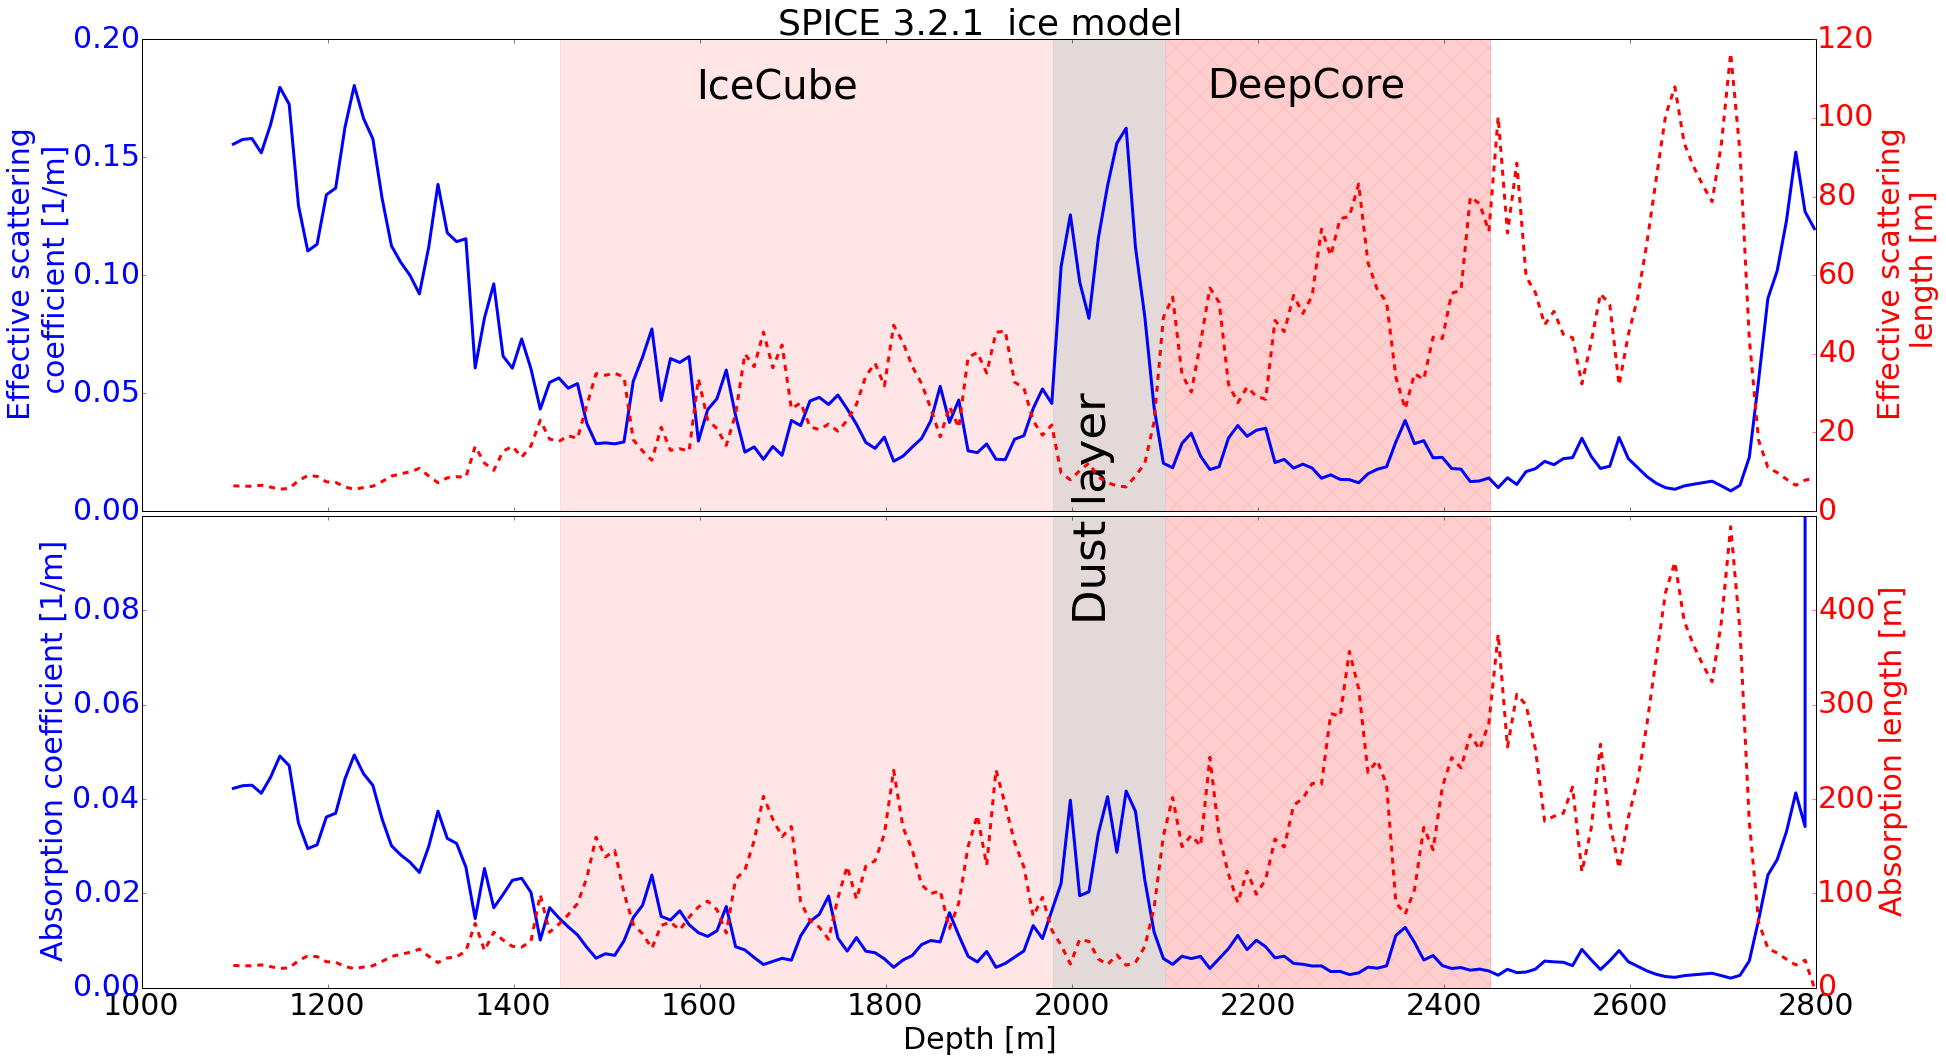
\includegraphics[width=0.9\linewidth]{figures/icecube/ice/Spice3.2.1_layered_scatt_abs_withlength_annotated.png}
    \caption{Scattering and absorption coefficients as a function of depth in the South Pole Ice (SPICE) model that is used to produce the simulation for this work.}
    \label{fig:spice-model}
\end{figure*}


\subsection{Simulation of Detector Response}

After the photons have reached the surface of the optical sensors, the simulation determines for each one if it is converted into a Monte-Carlo photo-electron (MCPE). The probability that this occurs depends on the wavelength-dependent sensitivity of the DOM, as well as the angular acceptance. The angular acceptance not only depends on the geometry of the DOM itself, but also incorporates the effect of the re-frozen column of ice surrounding each string. If a photon is accepted and converted into an MCPE, the next step is to simulate how much charge would be measured by the PMT inside the DOM as a response. The charge is drawn from a combination of a normal distribution and two exponential distributions whose parameters have been calibrated \emph{in-situ} to match the observed charge distribution in each individual DOM\sidecite{ic_spe_20}. This distribution, also referred to as the Single Photo-Electron (SPE) template, is shown in Figure~\ref{fig:spe-templates}. The MCPEs with the samples charge are then converted into simulated waveforms for the ATWD and fADC readouts which are then passed into the data processing chain starting from the \emph{wavedeform} algorithm described in Section~\ref{sec:dom-daq}. From there, the simulated events pass through all the same trigger and filter steps that are described in Section~\ref{sec:data-processing}.

\begin{figure}
    \centering
    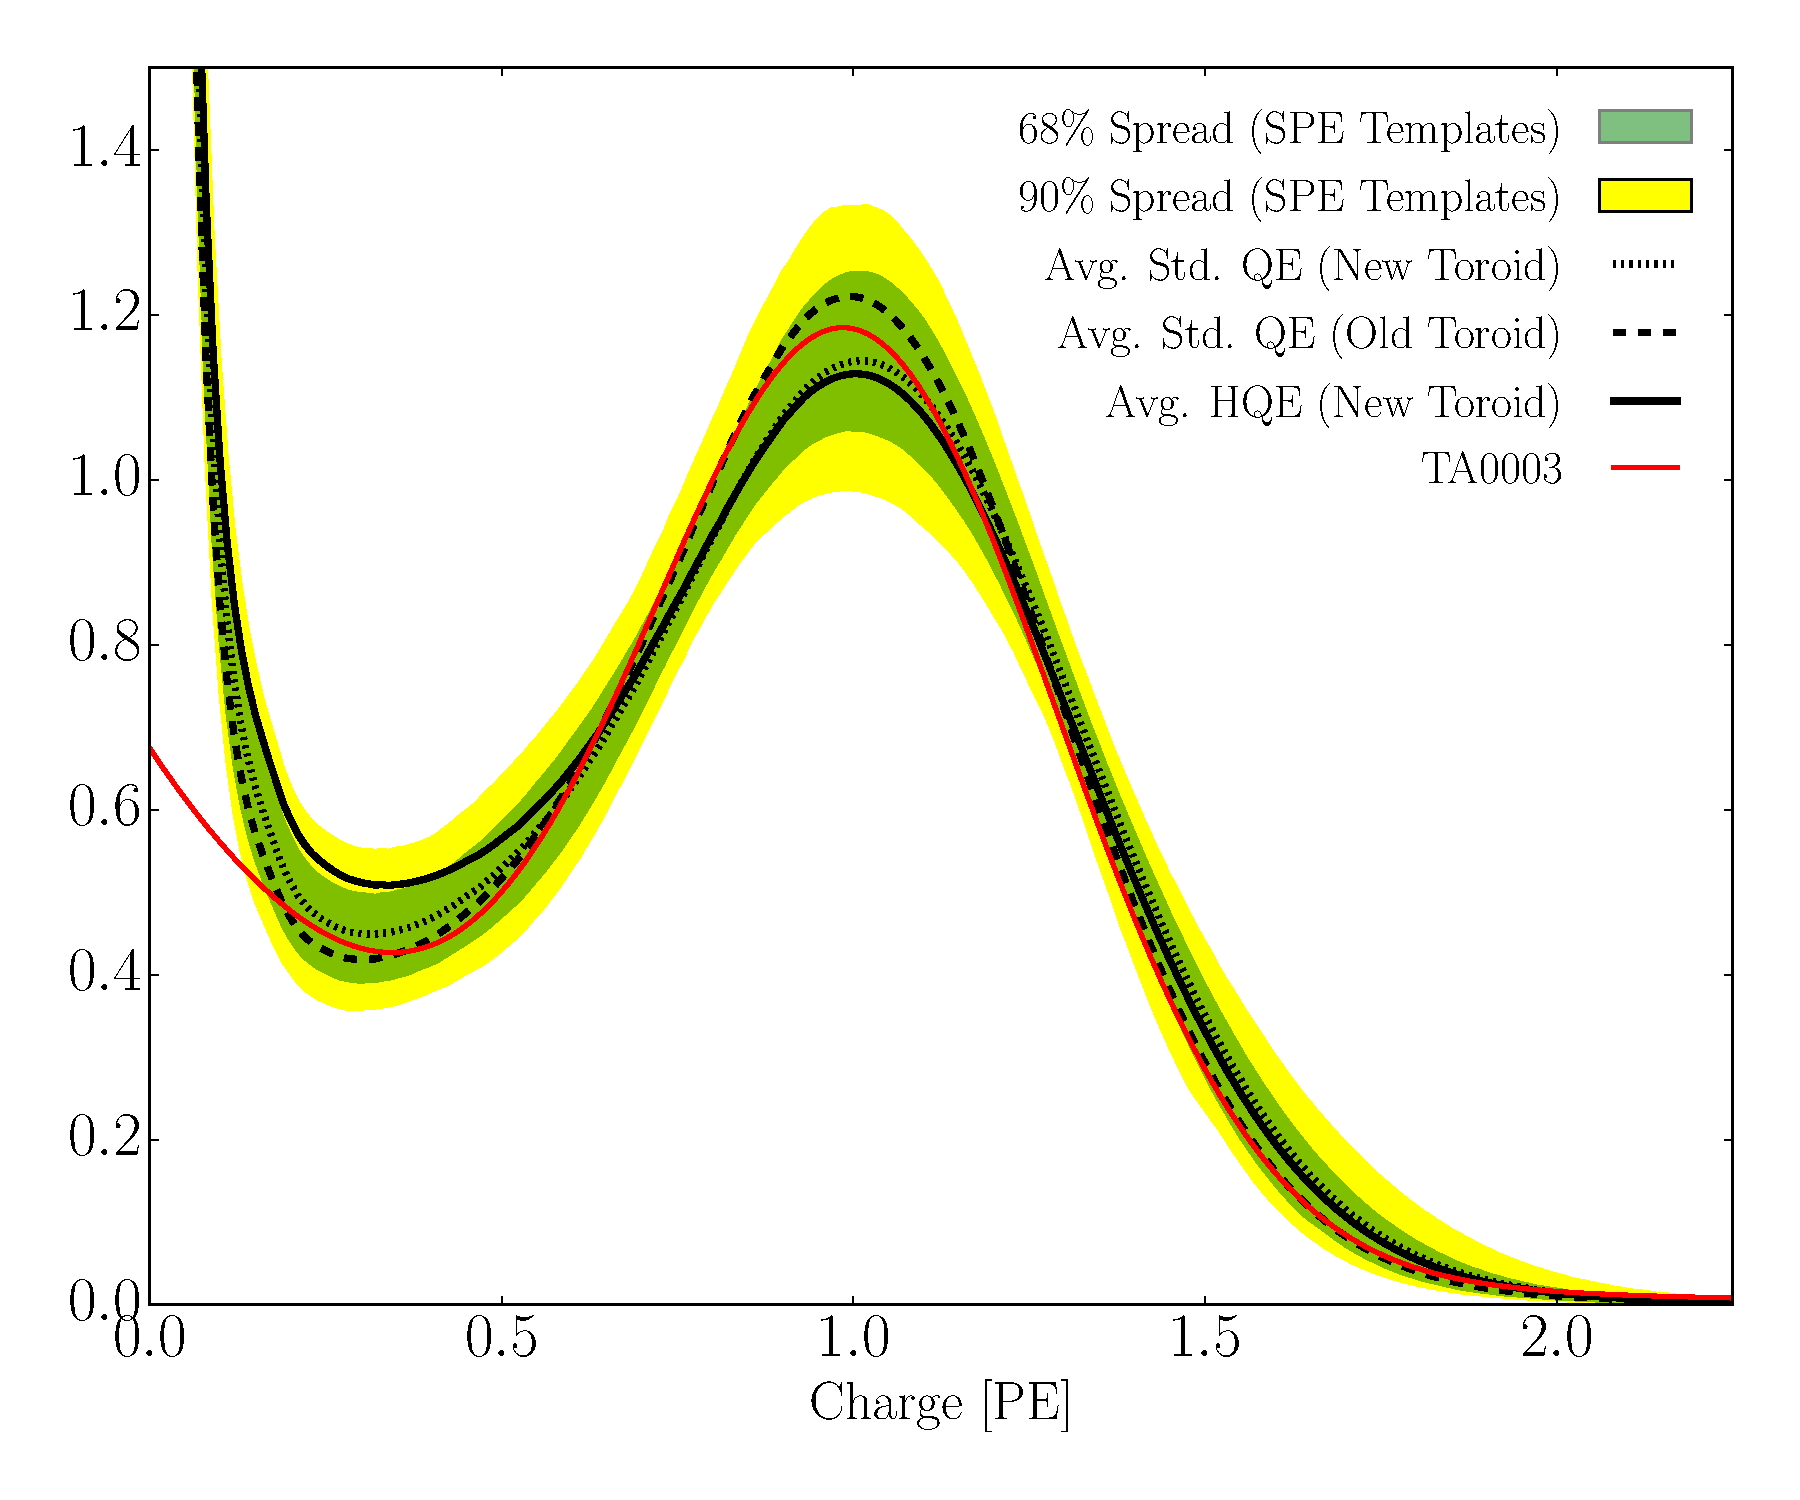
\includegraphics[width=0.8\linewidth]{figures/icecube/detector_response/SPE_TA003_2.pdf}
    \caption{The green (yellow) regions show the 68\% (90\%) spread in the SPE charge templates for a given charge.  Superimposed are the average SPE charge templates for the variety of hardware configurations shown in the black dotted, dashed, and solid lines. The TA0003 distribution, shown in red, originates from laboratory measurements. Figure taken from \cite{ic_spe_20}.}
    \label{fig:spe-templates}
\end{figure}

\subsubsection{Detector Noise}

\begin{margintable}
\caption{\label{tab:vuvuzela_params} Parameters used in the noise simulation. }
    \begin{tabular}{lc}\toprule
        \textbf{Parameter} & \textbf{Unit} \\ \midrule
        Thermal rate &  $s^{-1}$ \\ 
        Decay rate &  $s^{-1}$ \\
        Decay hits &  hits \\ 
        Decay hits mean &  $\log_{10} (ns) $\\ 
        Decay hits sigma &  $\log_{10} (ns) $ \\ \bottomrule
    \end{tabular}
\end{margintable}
Detector noise in IceCube consists mostly of photons produced in radioactive decay inside the glass housing of the DOMs and the PMTs. However, the simulation does not simulate the propagation of these photons. Instead, noise MCPEs are directly sampled from distributions that take both thermal and non-thermal noise components into account.The thermal component comes from uncorrelated photons and PMT dark noise and is modeled as a Poisson process with a constant rate. The non-thermal component comes from correlated bursts of photons that are produced by radioactive decays. To simulate it, decay times are first drawn from a Poisson process with a constant rate, and the number of photons produced in each event is sampled from a Poisson distribution. The time differences between the non-thermal MCPEs produced by each decay are then sampled from a Log-Gaussian distribution. This simulation method has five free parameters listed in Table~\ref{tab:vuvuzela_params} that are calibrated \emph{in-situ} for every DOM. All thermal and non-thermal MCPEs are injected into each simulated event together with the MCPEs from photons and passed into the rest of the simulation chain.
% \begin{margintable}
% \caption{\label{tab:vuvuzela_params} Parameters used in the noise simulation. }
%     \begin{tabular}{lcc}\toprule
%         \textbf{Parameter} & \textbf{Designation} & \textbf{Unit} \\ \midrule
%         Thermal rate & $\lambda_{Th}$ & $s^{-1}$ \\ 
%         Decay rate & $\lambda_{Decay}$ & $s^{-1}$ \\
%         Scintillation hits & $\eta_{Scint}$ & hits \\ 
%         Scintillation mean & $\mu_{Scint}$ & $\log_{10} (ns) $\\ 
%         Scintillation sigma & $\sigma_{Scint}$ &  $\log_{10} (ns) $ \\ \bottomrule
%     \end{tabular}
% \end{margintable}


\subsection{Final Sample and Binning}
\label{sec:sample-binning}
The starting point for this analysis is a DeepCore data sample consisting of 7.5 years of good live time and 21,914 events that pass through all selection steps described in section~\ref{sec:data-processing}. For every event in the sample, the energy and zenith angle is reconstructed as discussed in section~\ref{sec:event-reconstruction}. Both data and simulation sets are binned in reconstructed energy ($E_{\rm reco}$), cosine of the reconstructed zenith angle ($\cos(\theta_z)$), and PID as follows:

\begin{itemize}
    \item $E_{\rm reco}$: 11 bins spanning the range from 6.31~GeV to 158.49~GeV, the two bins with the highest energy are merged.
    \item $\cos(\theta_z)$: 10 bins spanning the range from -1 to 0.1
    \item PID: One bin between 0.55 and 0.75, and one bin between 0.75 and 1.0.
\end{itemize}

The lower PID bin between 0.55 and 0.75 consists to 69\%  (pre-fit MC estimate) of charged-current $\nu_\mu + \bar{\nu}_\mu$ events and is referred to as the \emph{mixed} channel, while the higher PID channel between 0.75 and 1.0 consists to 94\% of charged-current $\nu_\mu + \bar{\nu}_\mu$ events and is referred to as the \emph{tracks} channel. The histogram of both channels at the null hypothesis (i.e. no sterile signal) is shown in figure~\ref{fig:nominal-hist-null-hypo}.

\begin{figure}
    \centering
    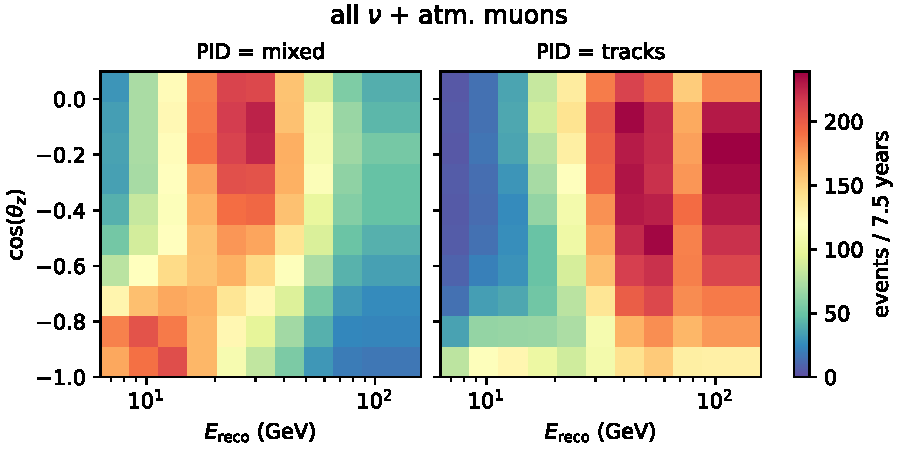
\includegraphics[width=0.95\textwidth]{figures/measurement/simulation_and_data/binning/plot_maps_total.pdf}
    \caption{Expected event counts in 7.5 years of live time assuming no sterile mixing and NuFit~4.0~\cite{nufit40} global best fit parameters at Normal Ordering.}
    \label{fig:nominal-hist-null-hypo}
\end{figure}

\begin{table}[htb]
\centering
\caption{Expected event rate with 8 years livetime broken down in event types and PID bins, calculated at NuFit~4.0 global best fit parameters.}
\label{tab:event-rate}
\begin{tabular}{lccc} \toprule
Type  & PID & Counts [8 years] & Rate [$\mathrm{\mu Hz}$] \\ \midrule
All MC & mixed  &   11428 &   48.3\\
All MC & tracks &   12238 &   51.7\\ \midrule
${\nu_{\rm all}} + {\bar\nu_{\rm all}} \, {\rm NC} $ & mixed  &     943 &    4.0 \\
${\nu_e} + {\bar\nu_e} \, {\rm CC}                 $ & mixed  &    1704 &    7.2 \\
${\nu_\mu} + {\bar\nu_\mu} \, {\rm CC}             $ & mixed  &    7901 &   33.4 \\
${\nu_\tau} + {\bar\nu_\tau} \, {\rm CC}           $ & mixed  &     470 &    2.0 \\
muons                                                & mixed  &     410 &    1.7 \\
\midrule
${\nu_{\rm all}} + {\bar\nu_{\rm all}} \, {\rm NC} $ & tracks &     171 &    0.7 \\
${\nu_e} + {\bar\nu_e} \, {\rm CC}                 $ & tracks &     294 &    1.2 \\
${\nu_\mu} + {\bar\nu_\mu} \, {\rm CC}             $ & tracks &   11517 &   48.7 \\
${\nu_\tau} + {\bar\nu_\tau} \, {\rm CC}           $ & tracks &     162 &    0.7 \\
muons                                                & tracks &      93 &    0.4 \\
\bottomrule
\end{tabular}
\end{table}

% \begin{figure*}
%     \centering
%     \ref{reco_coszen_prefit_legend}\par
%     \begin{tikzpicture}
    \pgfplotstableread{figures/icecube/selection/final_sample_prefit/reco_coszen.csv}\table
    \begin{groupplot}[
        xmin=-1.055,xmax=0.15500000000000003,
        xmode=normal,
        xmajorgrids, ymajorgrids,
        width=0.45\linewidth,
        ylabel style={at={(-0.15,0.5)}},
        group/.cd,
        group size=1 by 2,
        xticklabels at=edge bottom,
        vertical sep=10pt
        ]
    \nextgroupplot[
        height=0.3\linewidth,
        legend cell align={left},
        legend columns=-1,
        legend to name=reco_coszen_prefit_legend,
        ymode=log,
        ymin=2.670138976548827e-09, ymax=3e-5,
        ylabel=rate (Hz),
        ytick distance=1e1,
        % add magic filter to correctly handle empty bins in logarithmic y-axes:
        % If a bin-count is too low or zero, it would cause the line to be
        % interrupted, which creates artefacts and ugliness. Instead, we replace
        % these bin-counts with values that are just below the axis limit.
        % Because of the way pgfplots works, the input is the raw number but the
        % output has to be the log. Weird, I know.
        y filter/.expression={y < 2.670138976548827e-09 ? ln(2.6701389765488273e-10) : ln(y)}
    ]

    \ploterrorband[muon_color]{muon}{1}
    \addlegendentry{atm. muons}

    \ploterrorband[nue_color]{nuenuebar}{1}
    \addlegendentry{$\nu_e + \bar{\nu}_e$}

    \ploterrorband[numu_color]{numunumubar}{1}
    \addlegendentry{$\nu_\mu + \bar{\nu}_\mu$}

    \ploterrorband[nutau_color]{nutaunutaubar}{1}
    \addlegendentry{$\nu_\tau + \bar{\nu}_\tau$}


    % alternative event breakdown by interaction
    % \ploterrorband[nue_color]{nue_ccnuebar_cc}{1}
    % \addlegendentry{$\nu_e + \bar{\nu}_e$, CC}
    %
    % \ploterrorband[numu_color]{numu_ccnumubar_cc}{1}
    % \addlegendentry{$\nu_\mu + \bar{\nu}_\mu$, CC}
    %
    % \ploterrorband[nutau_color]{nutau_ccnutaubar_cc}{1}
    % \addlegendentry{$\nu_\tau + \bar{\nu}_\tau$, CC}
    %
    % \ploterrorband[nc_color]{nuall_ncnuallbar_nc}{1}
    % \addlegendentry{all $\nu$, NC}

    \ploterrorband{total_mc}{1}
    \addlegendentry{total MC}

    \ploterrorbar{data}
    \addlegendentry{data}

    \nextgroupplot[
        height=0.2\linewidth,
        ymin=-0.1, ymax=1.8,
        ylabel=rate/total MC,
        xlabel=reconstructed $\cos(\theta_{\mathrm{zenith}})$
    ]
   
    \ploterrorbar{data_mc_ratio}
    \plotratioerrorband[muon_color]{muon}{total_mc}
    \plotratioerrorband[nue_color]{nuenuebar}{total_mc}
    \plotratioerrorband[numu_color]{numunumubar}{total_mc}
    \plotratioerrorband[nutau_color]{nutaunutaubar}{total_mc}
    
    \end{groupplot}
\end{tikzpicture}

%     \tikzsetnextfilename{final_level_prefit_reco_energy}%
\begin{tikzpicture}
    \pgfplotstableread{figures/icecube/selection/final_sample_prefit/reco_energy.csv}\table
    \begin{groupplot}[
        xmin=5.362591587787688,xmax=185.61920737481475,
        xmode=log,
        xmajorgrids, ymajorgrids,
        width=0.45\linewidth,
        ylabel style={at={(-0.15,0.5)}},
        group/.cd,
        group size=1 by 2,
        xticklabels at=edge bottom,
        vertical sep=10pt
        ]
    \nextgroupplot[
        height=0.3\linewidth,
        legend cell align={left},
        legend columns=-1,
        legend to name=prefit_reco_energy_legend,
        ymode=log,
        ymin=2.670138976548827e-09, ymax=3e-5,
        ylabel=rate (Hz),
        ytick distance=1e1,
        % add magic filter to correctly handle empty bins in logarithmic y-axes:
        % If a bin-count is too low or zero, it would cause the line to be
        % interrupted, which creates artefacts and ugliness. Instead, we replace
        % these bin-counts with values that are just below the axis limit.
        % Because of the way pgfplots works, the input is the raw number but the
        % output has to be the log. Weird, I know.
        y filter/.expression={y < 9.437724466286084e-10 ? ln(9.437724466286085e-11) : ln(y)}
    ]

    \ploterrorband[muon_color]{muon}{1}
    \addlegendentry{atm. muons}

    \ploterrorband[nue_color]{nuenuebar}{1}
    \addlegendentry{$\nu_e + \bar{\nu}_e$}

    \ploterrorband[numu_color]{numunumubar}{1}
    \addlegendentry{$\nu_\mu + \bar{\nu}_\mu$}

    \ploterrorband[nutau_color]{nutaunutaubar}{1}
    \addlegendentry{$\nu_\tau + \bar{\nu}_\tau$}


    % alternative event breakdown by interaction
    % \ploterrorband[nue_color]{nue_ccnuebar_cc}{1}
    % \addlegendentry{$\nu_e + \bar{\nu}_e$, CC}
    %
    % \ploterrorband[numu_color]{numu_ccnumubar_cc}{1}
    % \addlegendentry{$\nu_\mu + \bar{\nu}_\mu$, CC}
    %
    % \ploterrorband[nutau_color]{nutau_ccnutaubar_cc}{1}
    % \addlegendentry{$\nu_\tau + \bar{\nu}_\tau$, CC}
    %
    % \ploterrorband[nc_color]{nuall_ncnuallbar_nc}{1}
    % \addlegendentry{all $\nu$, NC}

    \ploterrorband{total_mc}{1}
    \addlegendentry{total MC}

    \ploterrorbar{data}
    \addlegendentry{data}

    \nextgroupplot[
        height=0.2\linewidth,
        ymin=-0.1, ymax=1.8,
        ylabel=rate/total MC,
        xlabel=reconstructed energy (GeV)
    ]

    \ploterrorbar{data_mc_ratio}
    \plotratioerrorband[muon_color]{muon}{total_mc}
    \plotratioerrorband[nue_color]{nuenuebar}{total_mc}
    \plotratioerrorband[numu_color]{numunumubar}{total_mc}
    \plotratioerrorband[nutau_color]{nutaunutaubar}{total_mc}

    \end{groupplot}
\end{tikzpicture}

%     \caption{Distributions of reconstructed energy and zenith angle at the final level of the event selection, calculated assuming \textsc{NuFit}~4.0 global best fit oscillation parameters.}
%     \label{fig:pre-fit-energy-coszen}
% \end{figure*}
